\subsection{UC12: Gestione del carrello}
\label{sec:UC12}
\begin{figure}[!ht]
    \caption{Diagramma di UC12: Gestione del carrello}
    \vspace{10px}
    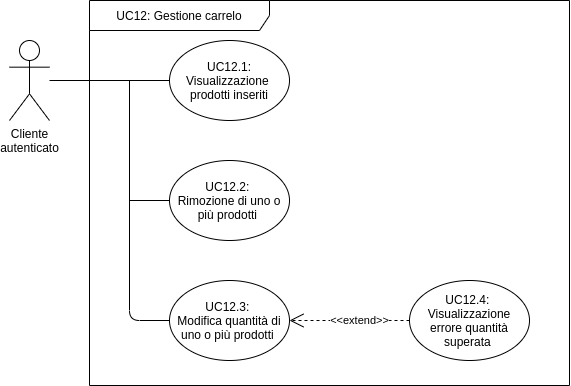
\includegraphics[scale=0.5]{../../../Images/AnalisiRequisiti/UC12}
    \centering
\end{figure}
\begin{itemize}
    \item \textbf{Descrizione:} questa sezione tratta l'insieme di operazioni che un utente generico compie per gestire i prodotti nel carrello;
    \item \textbf{Attore Primario:} utente generico;
    \item \textbf{Precondizione:} l'utente si trova in una qualsiasi pagina della piattaforma;
    \item \textbf{Input:} l'utente clicca il bottone per accedere alla pagina del carrello;
    \item \textbf{Postcondizione:} l'utente ha completato le operazioni per gestire i prodotti nel carrello;
    \item \textbf{Scenario Principale:}
          \begin{itemize}
              \item l'utente si trova in una qualsiasi pagina della piattaforma;
              \item l'utente clicca il bottone per accedere alla pagina del carrello;
              \item viene visualizzata la lista dei prodotti presenti nel carrello;
              \item l'utente può decidere se rimuovere qualche prodotto o modificarne la quantità.
          \end{itemize}
\end{itemize}
\subsubsection{UC12.1: Visualizzazione dei prodotti inseriti}
\label{sec:UC12.1}
\begin{itemize}
    \item \textbf{Descrizione:} sezione per visualizzare tutti i prodotti inseriti nel carrello;
    \item \textbf{Attore Primario:} utente generico;
    \item \textbf{Precondizione:}  l'utente si trova in una qualsiasi pagina della piattaforma;
    \item \textbf{Input:} l'utente clicca il bottone per accedere alla pagina del carrello;
    \item \textbf{Postcondizione:} l'utente visualizza la pagina del carrello e vede tutti i prodotti presenti al suo interno;
    \item \textbf{Scenario Principale:}
          \begin{itemize}
              \item l'utente si trova in una pagina della piattaforma;
              \item l'utente clicca il bottone per accedere alla pagina del carrello;
              \item l'elenco dei prodotti presenti nel carrello è visibile a schermo.
          \end{itemize}
\end{itemize}
\subsubsection{UC12.2: Rimozione di uno o più prodotti}
\label{sec:UC12.2}
\begin{itemize}
    \item \textbf{Descrizione:} sezione per rimuovere uno o più prodotti dal carrello;
    \item \textbf{Attore Primario:} utente generico;
    \item \textbf{Precondizione:} l'utente è nella pagina del carrello (\hyperref[sec:UC12.1]{\underline{UC12.1}});
    \item \textbf{Input:} l'utente seleziona i prodotti da rimuovere dal carrello;
    \item \textbf{Postcondizione:} vengono rimossi i prodotti selezionati;
\end{itemize}
\subsubsection{UC12.3: Modifica della quantità di uno o più prodotti}
\label{sec:UC12.3}
\begin{itemize}
    \item \textbf{Descrizione:} sezione per modificare la quantità dei prodotti nel carrello;
    \item \textbf{Attore Primario:} utente generico;
    \item \textbf{Precondizione:} l'utente è nella pagina del carrello (\hyperref[sec:UC12.1]{\underline{UC12.1}});
    \item \textbf{Input:} l'utente seleziona la nuova quantità desiderata per i prodotti;
    \item \textbf{Postcondizione:} le modifiche sono applicate;
    \item \textbf{Estensioni:}
          \begin{itemize}
              \item se la quantità inserita dovesse superare la quantità disponibile, l'utente viene avvisato (\hyperref[sec:UC12.4]{\underline{UC12.4}}).
          \end{itemize}
\end{itemize}
\subsection{UC12.4 Visualizzazione errore quantità superata}
\label{sec:UC12.4}
\begin{itemize}
    \item \textbf{Descrizione:} la quantità inserita dall'utente supera quella disponibile in magazzino;
    \item \textbf{Attore primario:} utente generico;
    \item \textbf{Precondizione:} l'utente si trova all'interno del carrello;
    \item \textbf{Postcondizione:} viene visualizzato il messaggio di errore.
\end{itemize}